
\section{Systematic Uncertainties with binning used in Pb-Pb analsyis}

We considered the following sources of systematic uncertainties:

\begin{easylist}[itemize]
& Raw yield extraction
& D-Meson Selection Cuts
& B Feed-Down
& Unfolding and background fluctuation matrix
& Tracking Efficiency
& \pt\ Shape of the Monte Carlo Spectrum
\end{easylist}

\subsection{Raw Yield Extraction}
The stability and systematics of the raw yield extraction has been assessed using the \texttt{MultiTrial} framework developed by the D2H group.
This framework performs the fit of the invariant mass distribution many times varying several conditions, such us binning, fixed vs. free parameters, background function, fit range.

\subsubsection{\Dzero-tagged jets}

The following variations were included in the assessment of the systematics for the raw yield extraction of \Dzero jets in \pPb:
\begin{itemize}
\item fixed $\sigma=\sigma_{\rm MC}$;
\item fixed $\sigma=1.15\sigma_{\rm MC}$
\item fixed $\sigma=0.85\sigma_{\rm MC}$
\item free $\sigma$ and fixed $m_{0}=m_{\rm PDG}$;
\item fixed $\sigma=\sigma_{\rm MC}$ and $m_{0}=m_{\rm PDG}$;
\item free $\sigma$ and free $m_{0}$;
\item background functions: exponential, linear, second-order polynomial;
\item lower limit of fit range: $1.72$, $1.74$~\GeVcsq;
\item upper limit of fit range: $2.00$, $2.03$~\GeVcsq;
\item rebin by factor 2
\end{itemize}


Figure~\ref{fig:PbPb_MultiTrialSB_trials_pPB_Dzero} shows average of the multi-trial procedure for the side-band method as a function of jet \pt\ for each \Dzero \pt\ bin scaled by the corresponding efficiency, and average of the all \Dzero\ \pt\ bins (blue). 
Variations of all trials as a function of jet \pt\ for each \Dzero\ \pt\ bin and scaled by the corresponding efficiency are shown in Fig~\ref{fig:PbPb_MultiTrialSB_allDptVairations_pPB_Dzero}.


The systematic uncertainties are calculated as the root-mean-square of all the yields obtained in the multi-trial fits and are shown in Fig.~\ref{fig:PbPb_MultiTrialRMS_pPB_Dzero}.
\begin{figure}[bth]
\begin{center}
\includegraphics[width=0.5\textwidth]{pPbplotsD0/Default_jetMeas3_50_jetTrue3_50_PbPbbinning/systematics/YieldExtSysUnc_SB.pdf}
\caption{\Dzero-jet systematic uncertanties, RMS.} 
\label{fig:PbPb_MultiTrialRMS_pPB_Dzero}
\end{center}
\end{figure}


\textbf{Variation of signal and side-band ranges}

As an additional systematic unceratnty, variations of ranges of the signal and side-band definitions in the invariant-mass fit procedure are considered.
Figure~\ref{fig:PbPb_JetPtSys_Dzero_SBvariaton} shows ratios of efficiency and B feed-down corrected yields to the central value and RMS of the variations.

\begin{figure}[bth]
\begin{center}
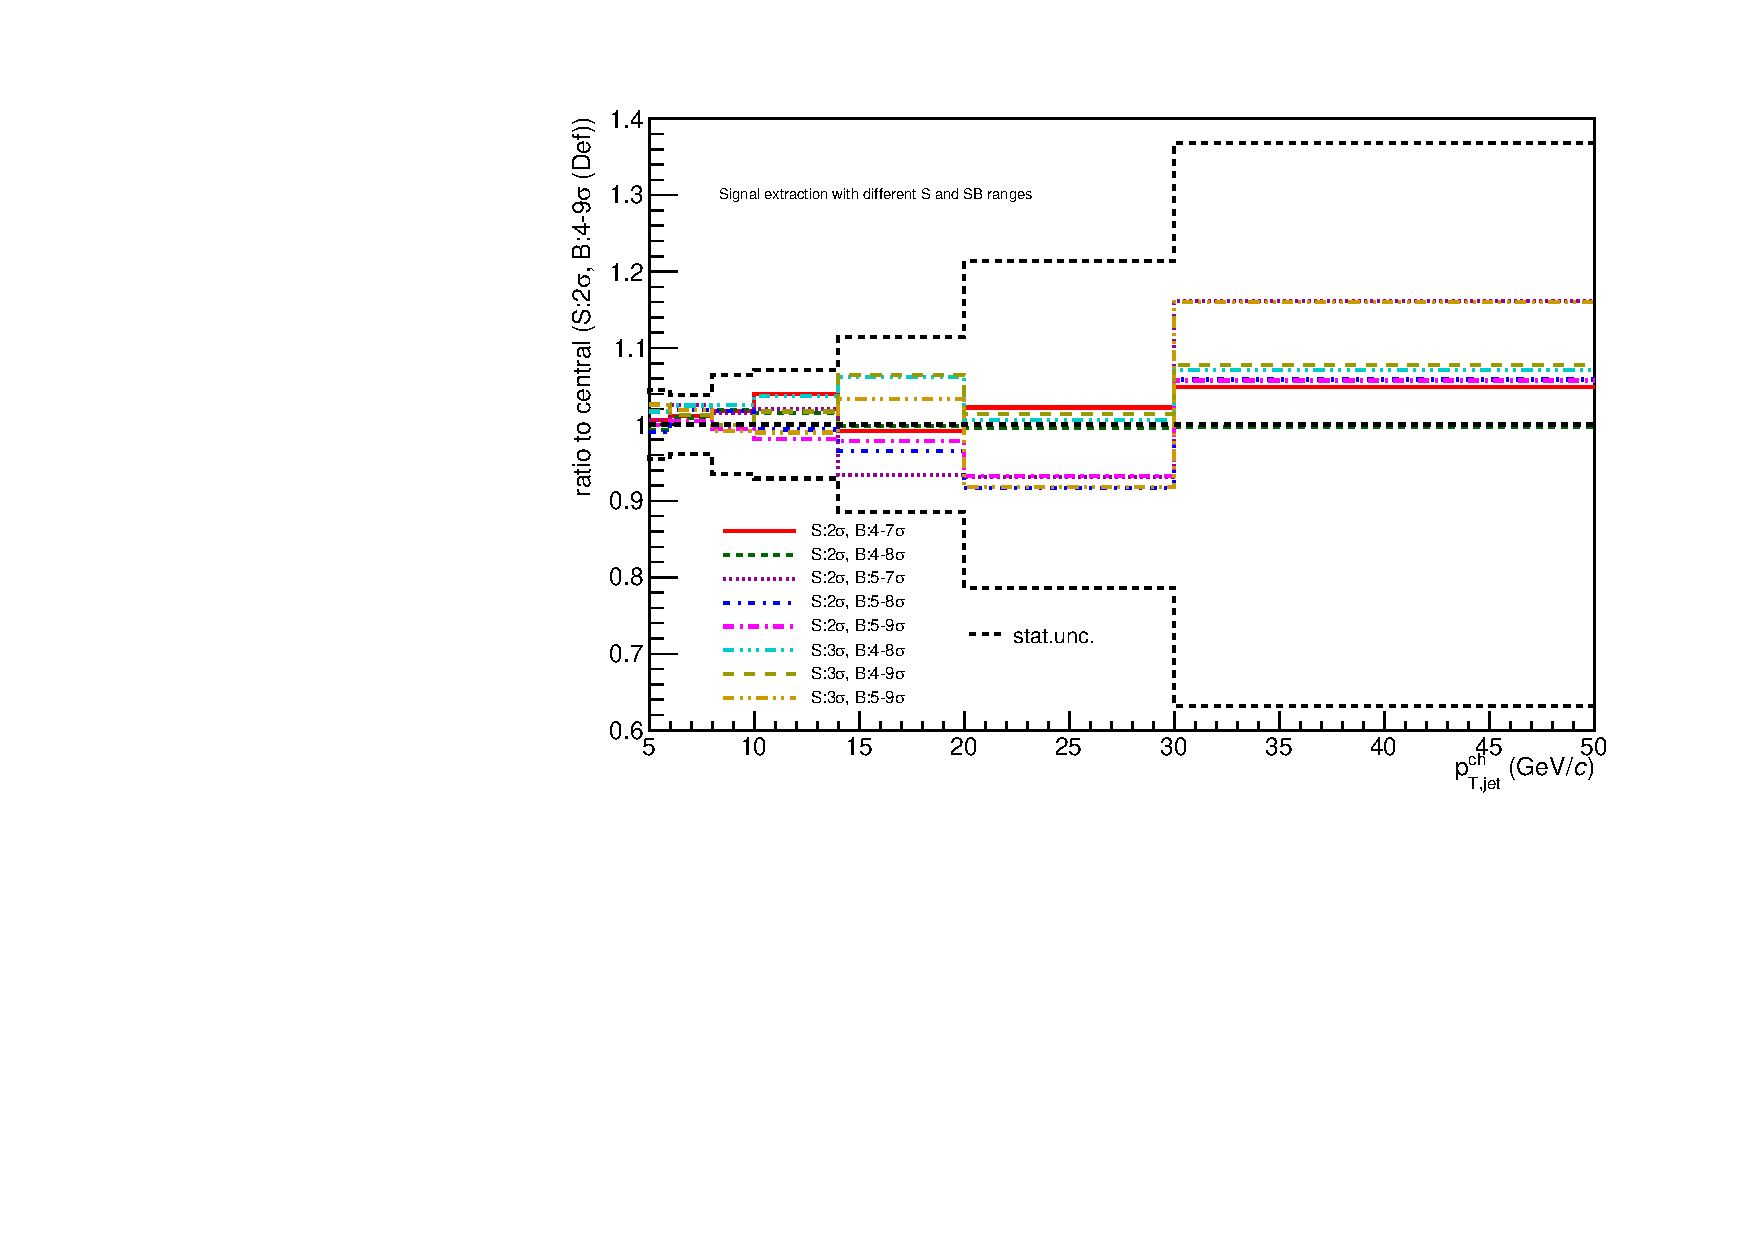
\includegraphics[width=0.49\textwidth]{pPbplotsD0/Default_jetMeas3_50_jetTrue3_50_PbPbbinning/systematics/SBRangesComparison_ratio.pdf}
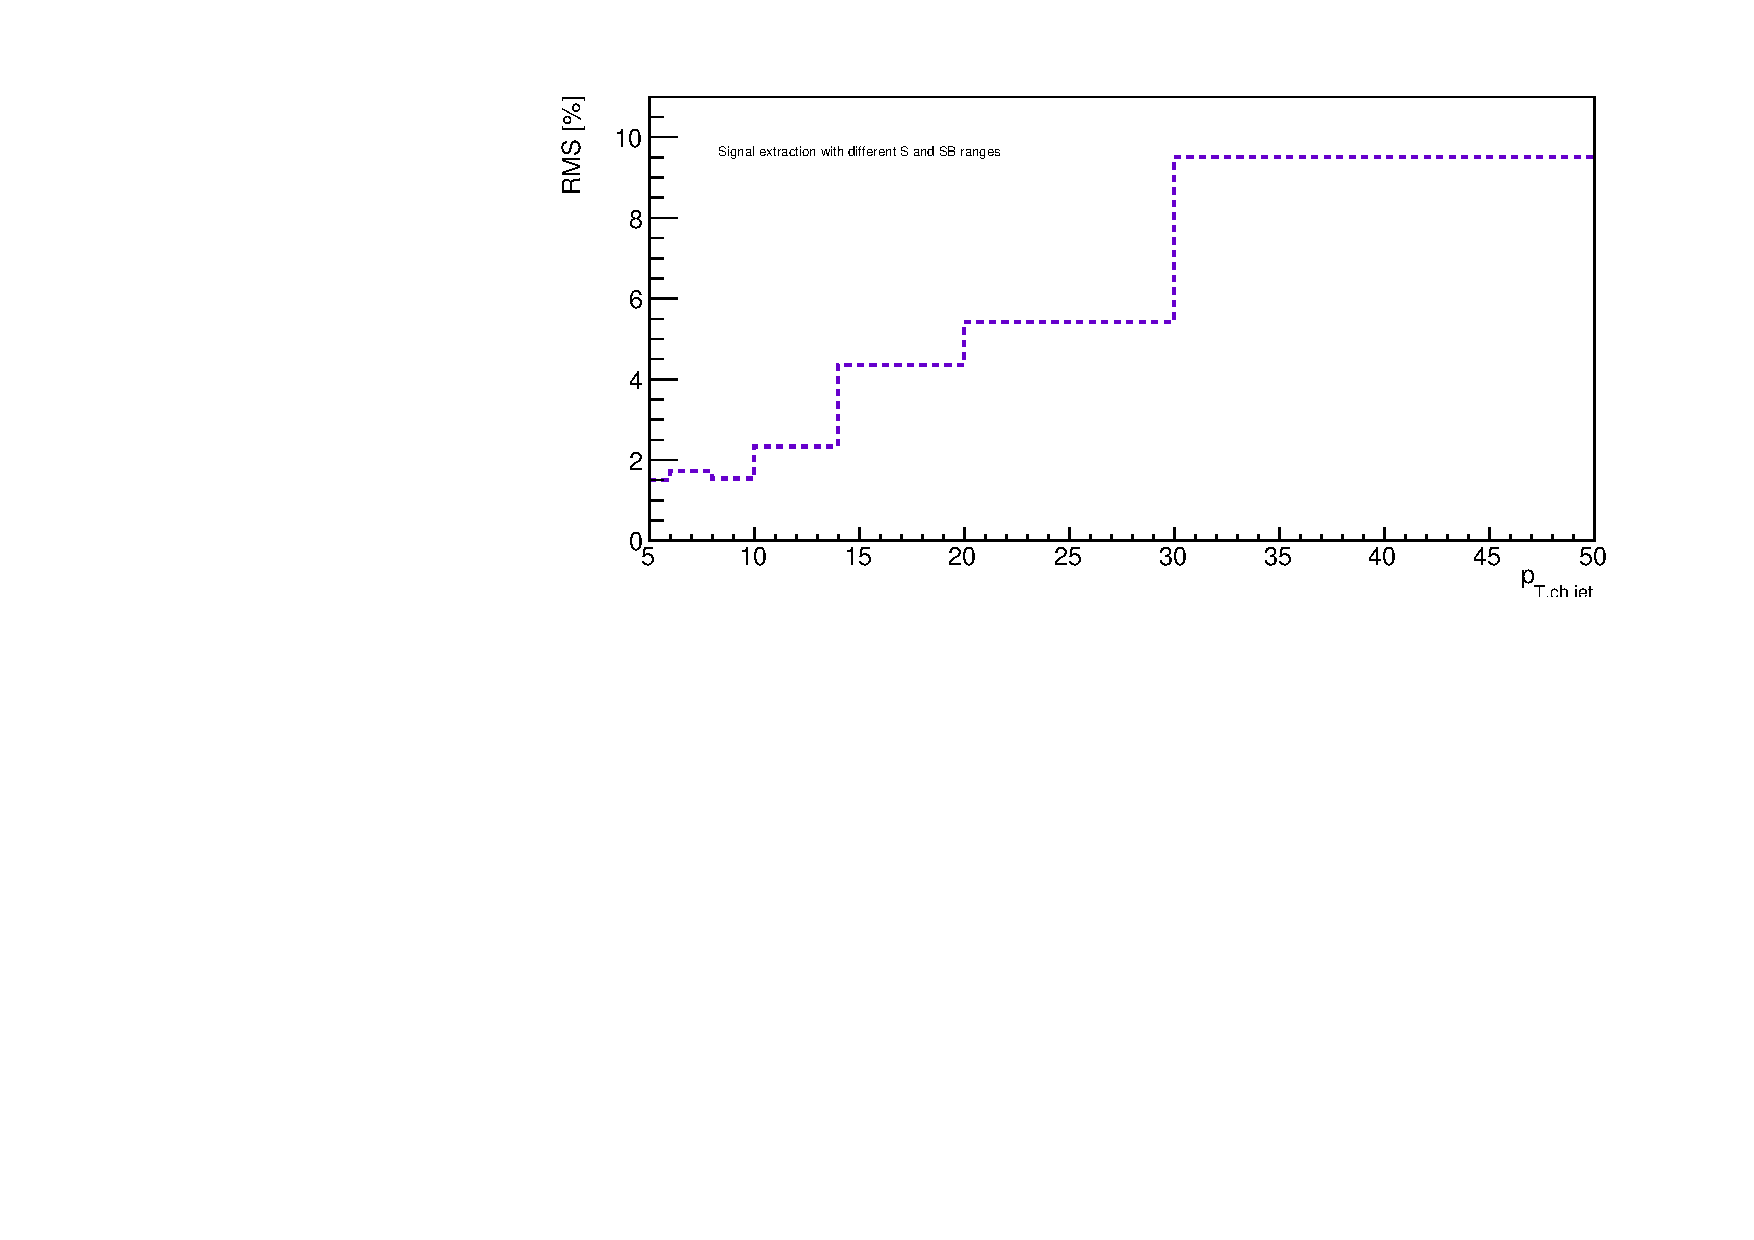
\includegraphics[width=0.49\textwidth]{pPbplotsD0/Default_jetMeas3_50_jetTrue3_50_PbPbbinning/systematics/SBRangesComparison_rms.pdf}
\caption{\Dzero-jet. Left:Systematic unceratnties from the variation of definitions of the signal and side-band regions. Right: Systematic uncertanty: RMS.} 
\label{fig:PbPb_JetPtSys_Dzero_SBvariaton}
\end{center}
\end{figure}


\textbf{Variation of reflection to signal ratio}

By default, the ratio reflection/signal is a fixed parameter in the fit and is taken from the MC simulation. The reflection/signal ratio is varied to estimate the
systematic uncertainty. Consider variations are $\pm$ 50\% of the default value. Systematic uncertanties arising from these variation on the final unfolded jet \pt\ spectra are 1-3\%, as shown in Fig.~\ref{fig:PbPb_JetPtSys_Dzero_Refl}.

\begin{figure}[bth]
\begin{center}
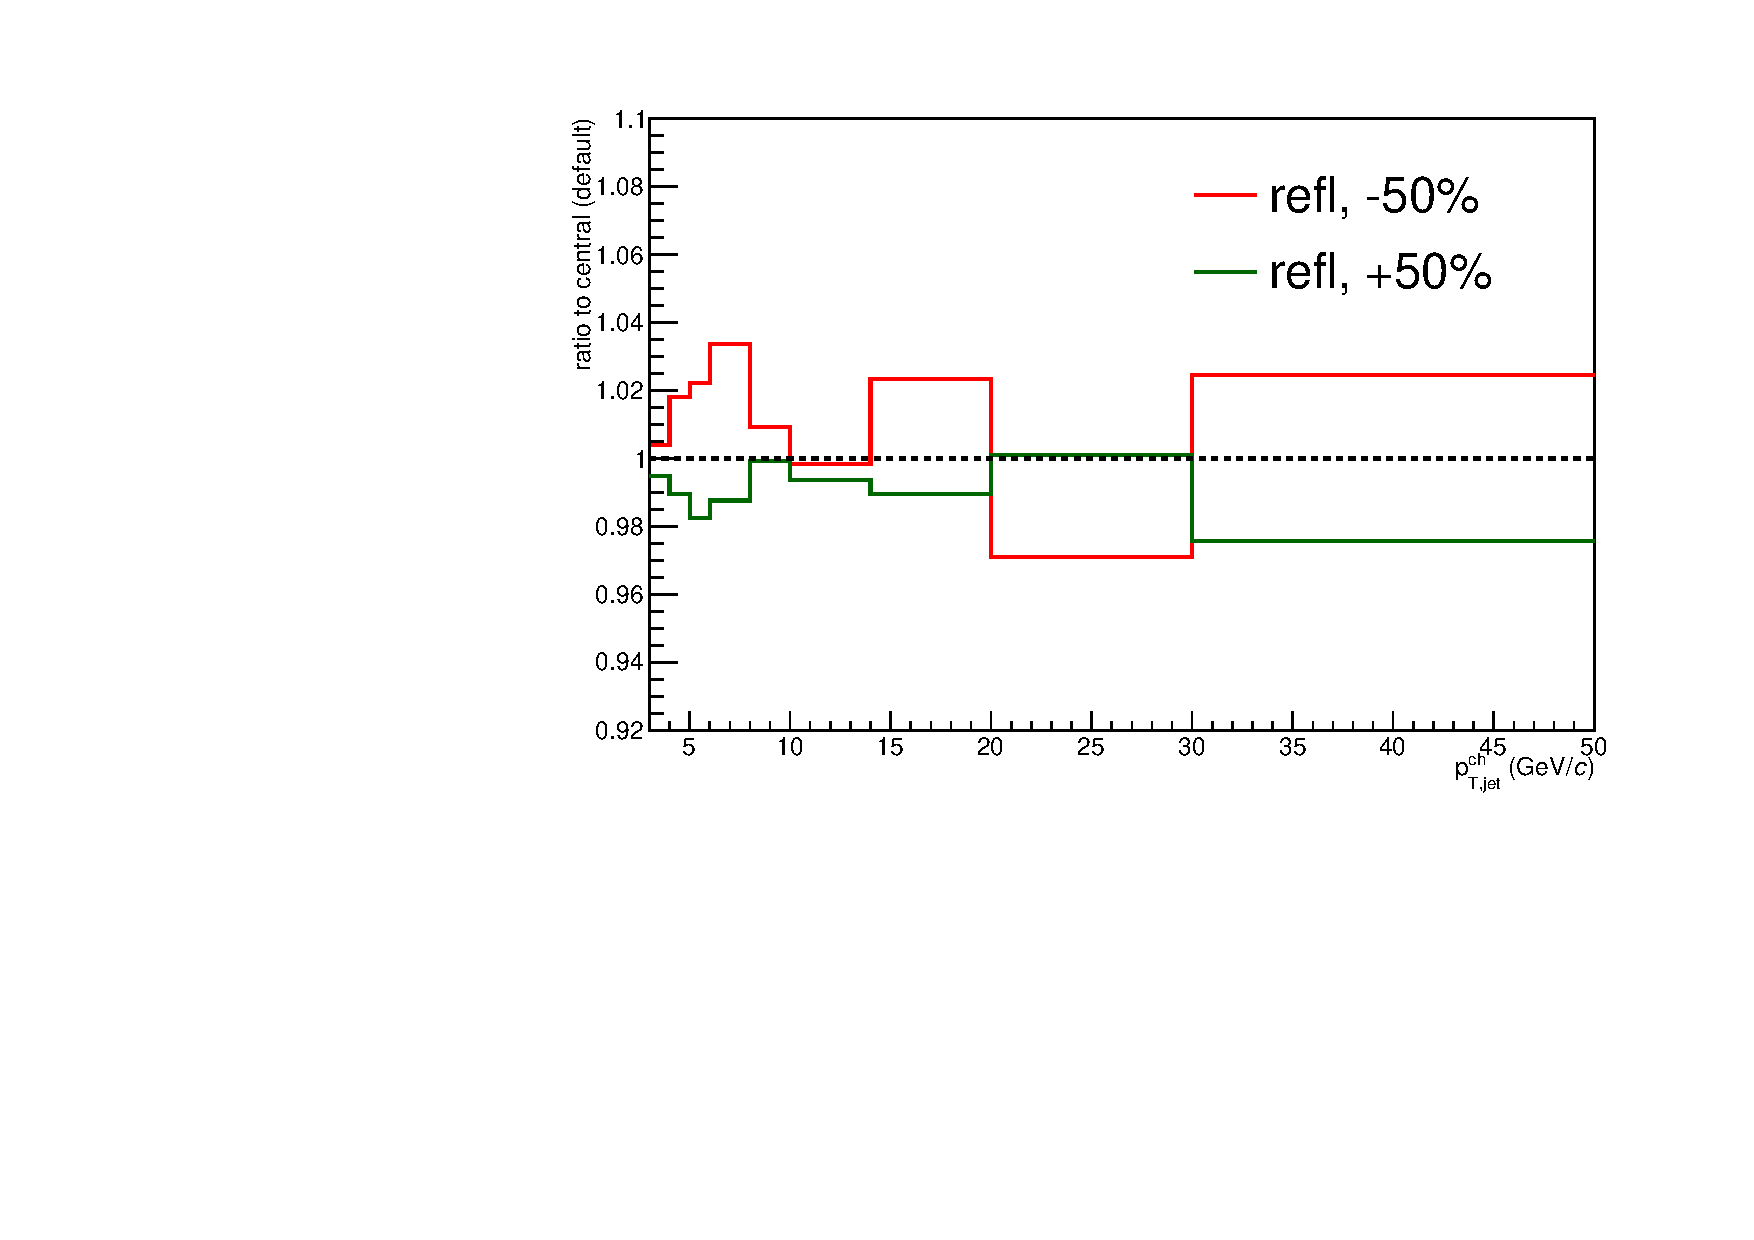
\includegraphics[width=0.49\textwidth]{pPbplotsD0/Default_jetMeas3_50_jetTrue3_50_PbPbbinning/systematics/RawYield_reflections_ratio.pdf}
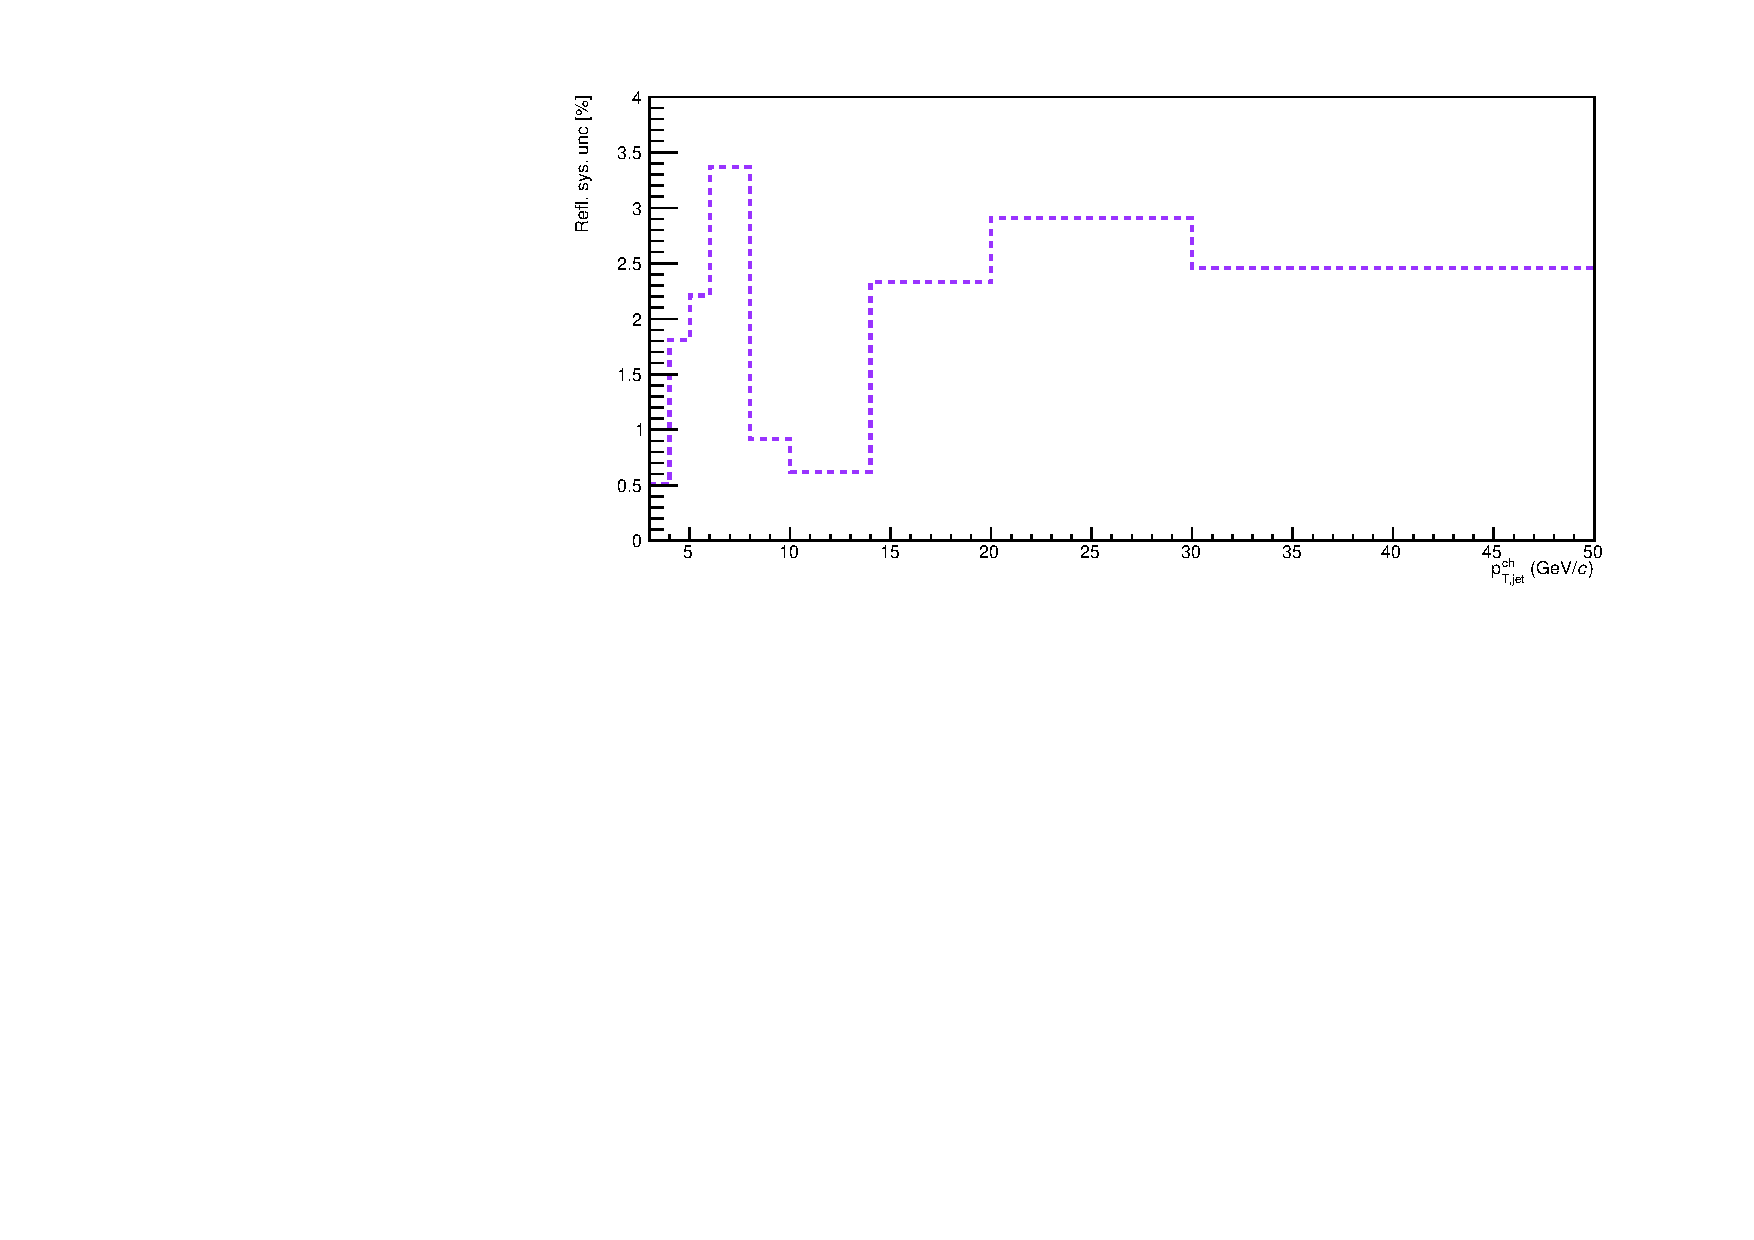
\includegraphics[width=0.49\textwidth]{pPbplotsD0/Default_jetMeas3_50_jetTrue3_50_PbPbbinning/systematics/RawYield_reflections_sys.pdf}
\caption{\Dzero-jet. Left:Ratio of unfolded jet \pt\ spectrum with $\pm$ 50\% variatitions of the reflection/signal ratio. Right: Systematic uncertanity, maximum of the variations in each bin.} 
\label{fig:PbPb_JetPtSys_Dzero_Refl}
\end{center}
\end{figure}


The uncertanties are added in quadratures in order to obtain the final systematic uncertainty on the raw yield extraction. 

\subsection{D-Meson Selection Cuts}
Uncertainties of the D-meson cut selection is estimated by varying applied in the analysis D-meson selection criteria, as reported in~\ref{sec:DmesonSel}. 


\subsubsection{\Dzero-tagged jets}

7 variations of cut selection are considered, 4 looser sets and 3 tighter sets of cuts. The variations are choosen so that they vary \Dzero reconstruction efficiency to high enough extend so that a possible imperfection in MC simulation can be probe. Though at high \ptd\ the selection criteria are already rather loose.
Raw \Dzero-jet \pt\ distributions with these different cut sets and corresponding \Dzero-jet efficiencies are shown in Fig.~\ref{fig:PbPb_JetPtRawSys_Dzero}, and ratios to the default set of cuts in Fig.~\ref{fig:PbPb_JetPtRawSysRatio_Dzero}.
Figure~\ref{fig:PbPb_JetcutVarFD_Dzero} shows non-prompt \Dzero-jet reconstruction efficiencies for all the cut variations, and the variations of the FD fraction in the inclusive \Dzero-jet spectrum.

\begin{figure}[bth]
\begin{center}
\includegraphics[width=0.49\textwidth]{pPbplotsD0/Default_jetMeas3_50_jetTrue3_50_PbPbbinning/systematics/CutVariationSyst_reg0_RawSpectra.pdf}
\includegraphics[width=0.49\textwidth]{pPbplotsD0/Default_jetMeas3_50_jetTrue3_50_PbPbbinning/systematics/CutVariationSyst_reg0_PromptEfficiencies.pdf}
\caption{\Dzero-jet. Left: \Dzero-jet \pt\ distributions with different cut sets for systematic uncertainties estimation. Right: corresponding prompt \Dzero-jet efficiencies.} 
\label{fig:PbPb_JetPtRawSys_Dzero}
\end{center}
\end{figure}

\begin{figure}[bth]
\begin{center}
\includegraphics[width=0.49\textwidth]{pPbplotsD0/Default_jetMeas3_50_jetTrue3_50_PbPbbinning/systematics/CutVariationSyst_reg0_RawSpectra_ratio.pdf}
\includegraphics[width=0.49\textwidth]{pPbplotsD0/Default_jetMeas3_50_jetTrue3_50_PbPbbinning/systematics/CutVariationSyst_reg0_PromptEfficiencies_ratio.pdf}
\caption{\Dzero-jet. Left: Ratios of \Dzero-jet \pt\ distributions with different cut sets for systematic uncertainties estimation. Right: ratios of the corresponding \Dzero-jet efficiencies.} 
\label{fig:PbPb_JetPtRawSysRatio_Dzero}
\end{center}
\end{figure}

\begin{figure}[bth]
\begin{center}
\includegraphics[width=0.49\textwidth]{pPbplotsD0/Default_jetMeas3_50_jetTrue3_50_PbPbbinning/systematics/CutVariationSyst_reg0_NonPromptEfficiencies_ratio.pdf}
\includegraphics[width=0.49\textwidth]{pPbplotsD0/Default_jetMeas3_50_jetTrue3_50_PbPbbinning/systematics/CutVariationSyst_reg0_FDFraction_ratio.pdf}
\caption{\Dzero-jet. Ratios of \Dzero-jet non-prompt reconstruction efficiencies (left) and FD fractions (right) with different cut sets for systematic uncertainties estimation.} 
\label{fig:PbPb_JetcutVarFD_Dzero}
\end{center}
\end{figure} 

Corrected for the corresponding efficiency \Dzero-jet \ptchjet\ distributions are presented in Fig.~\ref{fig:PbPb_JetPtSys_Dzero}. Systematic uncertainties are estimated by taking ratio of the efficiency-corrected, FD subtracted and unfolded \Dzero-jet \ptchjet\ distributions with different cut variations to the \Dzero-jet \pt\ spectrum obtained with the default cut set and taking RMS of them, as shown in Fig.~\ref{fig:PbPb_JetPtSys_Dzero}.

\begin{figure}[bth]
\begin{center}
\includegraphics[width=0.49\textwidth]{pPbplotsD0/Default_jetMeas3_50_jetTrue3_50_PbPbbinning/systematics/CutVariationSyst_reg0_CorrectedSpectra.pdf}
\caption{\Dzero-jet. Efficiency-corrected, FD subtracted and unfolded \Dzero-jet \pt\ distributions with different cut sets for systematic uncertainties estimation.} 
\label{fig:PbPb_JetPtSys_Dzero}
\end{center}
\end{figure}

\begin{figure}[bth]
\begin{center}
\includegraphics[width=0.49\textwidth]{pPbplotsD0/Default_jetMeas3_50_jetTrue3_50_PbPbbinning/systematics/CutVariationSyst_reg0_CorrectedSpectra_ratio.pdf}
\includegraphics[width=0.49\textwidth]{pPbplotsD0/Default_jetMeas3_50_jetTrue3_50_PbPbbinning/systematics/CutVariationSyst_reg0_CorrectedSpectra_rms.pdf}
\caption{\Dzero-jet. Left: Ratio of the efficiency-corrected \Dstar-jet \pt\ distributions with different cut sets for systematic uncertainties estimation. Right: RMS - systematic uncertainties.} 
\label{fig:PbPb_JetPtSys_Dzero}
\end{center}
\end{figure}


As a cross-check, systematics from cut variation were also extracted using different definitions of signal and side-band regions in the invariant mass fitting procedure. Comparison of the systematic uncertanties obtained from these variatons and mean of them in shown in Fig.~\ref{fig:PbPb_JetPtSys_Dzero_SB}. The high jet \pt\ bins are influenced by a statistical unceratnties from the background fluctuations. 

\begin{figure}[bth]
\begin{center}
\includegraphics[width=0.49\textwidth]{pPbplotsD0/Default_jetMeas3_50_jetTrue3_50_PbPbbinning/systematics/SBRangesComparisonCutSys.pdf}
\includegraphics[width=0.49\textwidth]{pPbplotsD0/Default_jetMeas3_50_jetTrue3_50_PbPbbinning/systematics/SBRangesComparisonCutSys_mean.pdf}
\caption{\Dzero-jet. Left:Systematic unceratnties from the cut variation with different definitions of the signal and side-band regions. Right: Mean.} 
\label{fig:PbPb_JetPtSys_Dzero_SB}
\end{center}
\end{figure}

\subsection{B Feed-Down Correction}

The B Feed-Down (FD) cross section is obtained from a POWHEG+PYTHIA6 simulation, as discussed in Section~\ref{sec:FD}.
In order to assess the systematic uncertainty the same simulation is performed with different choices of the quark mass $m_{\rm b}$, the factorization scale factor $\mu_{\rm F}$, and the renormalization scale factor $\mu_{\rm R}$.
Table~\ref{tab:FDpars} shows the list of parameters used to determine the central points and the variations used to determine the systematic uncertainty.


\begin{table}[bth]
\caption{Parameters of the POWHEG+PYTHIA6 simulations used to estimate the B Feed-Down.}
     \label{tab:FDpars}
\begin{center}
    \begin{tabular}{lrr}
    \hline
    Parameter & Central Value & Variations \\ \hline
    $m_{\rm b}$ & $4.75$~\GeVcsq & $4.5$, $5.0$~\GeVcsq \\ 
    PDF & CT10nlo (11000) & -- \\ 
    nPDF & EPS09nlo & -- \\
    ($\mu_{\rm F}$, $\mu_{\rm R}$) & (1,1) & (0.5,0.5), (0.5, 1), (1, 0.5), (2,2), (2,1), (1,2)
    \end{tabular}
    \end{center}
    \end{table}

\subsubsection{\Dzero-tagged jets}

In the case of \Dzero-jet analysis, an additional variation is considered: an EvtGen is used as a decayer instead of Pytha6. \ptchjet\ \pt\ differential cross-section for B $\rightarrow$ \Dzero\ for all the variations and ratios to the default cross-section are shown in  in Fig.~\ref{fig:PbPb_BFeedDown_JetPtSpectrum_Dzero}.
The \ptchjet\ distribution is with the analysis cut on 3 $< \ptd <$ 36 GeV/$c$, ratios before scaling by non-prompt to prompt efficiency are shown in Fig.~\ref{fig:PbPb_BFeedDown_JetPtSpectrum_Dzero}.


\begin{figure}[bth]
\begin{center}
\includegraphics[width=.45\textwidth]{pPbplotsD0/Simulations/BFeedDown/plots/NonPromptspectra_JetPt_Dpt3_36.pdf}
\includegraphics[width=.45\textwidth]{pPbplotsD0/Simulations/BFeedDown/plots/NonPromptspectra_JetPt_Dpt3_36_ratio.pdf}
\caption{Non-prompt (B Feed-Down) \Dzero-jet cross section in \pPb\ at $\snn=5.02$~TeV as a function of \ptchjet, obtained in POWHEG+PYTHIA6 simulations
with different choices of the simulation parameters, \ptd\: 3-36 GeV/$c$.} 
\label{fig:PbPb_BFeedDown_JetPtSpectrum_Dzero}
\end{center}
\end{figure}

The non-prompt \Dzero-jet \pt\ spectrum after correcting for the efficiency and smearing with the detector effects is shown in Fig.~\ref{fig:PbPb_pPbFD_corr_Dzero}, together with systematic uncertainties obtained by taking the largest upward and downward variation from the central point in each bin,therefore the shown uncertainties are asymmetric (see left panel of Fig.~\ref{fig:PbPb_BFeedDown_sysUnc_Dzero}). AS the FD subtraction systematic uncertainty the largest between the upward and downward uncertainty is used in order to have a symmetric uncertainty, as shown in Fig.~\ref{fig:PbPb_BFeedDown_sysUnc_Dzero}.

\begin{figure}[bth]
\begin{center}
\includegraphics[width=.49\textwidth]{pPbplotsD0/Default_jetMeas3_50_jetTrue3_50_PbPbbinning/systematics/FD_reg3_ratio.pdf}
\includegraphics[width=.49\textwidth]{pPbplotsD0/Default_jetMeas3_50_jetTrue3_50_PbPbbinning/systematics/FD_reg3_unc.pdf}
\caption{Systematic uncertainties on the unfolded \Dzero-jet \pt\ spectrum from the B feed-down subtraction.} 
\label{fig:PbPb_BFeedDown_sysUnc_Dzero}
\end{center}
\end{figure}


\subsection{Unfolding}
\label{sUnfoldSys}

\subsubsection{\Dzero-tagged jets}

Unfolded \Dzero-jet \pt\ spectrum using the Bayesian method with 3 iteration was shown in Fig.~\ref{fig:PbPb_UnfSpec_pPb_Dzero}, and the evolution of \Dzero-jet spectrum in \pPb\ collisions increasing number of iterations compare to Bayesian unfolding with 3 iterations was shown in Fig.~\ref{fig:PbPb_unfIterations_pPb_Dzero}. 
The default \ptchjet\ ranges for the unfolding procedure are 3 $< \ptchjet< $ 50 both at the generator and reconstructed level \pt\, with over/under flow bins considered in the unfolding procedure, where $p_{T,jet}^{reco}$ is also the range of the measured in the data \Dzero-jet \pt\ spectrum being unfolded. 
As systematic checks these ranges are varied.
Additional check of the unfolding was done by performing unfolding using the SVD algoritm wiht $reg=6,7$.
All these checks are summarized in Fig.~\ref{fig:PbPb_UnfSpec_pPb_Dzero_ranges} as ratios of the unfolded spectra to the default case. The assign systematic uncerantity is from the RMS.

\begin{figure}[bth]
\centering
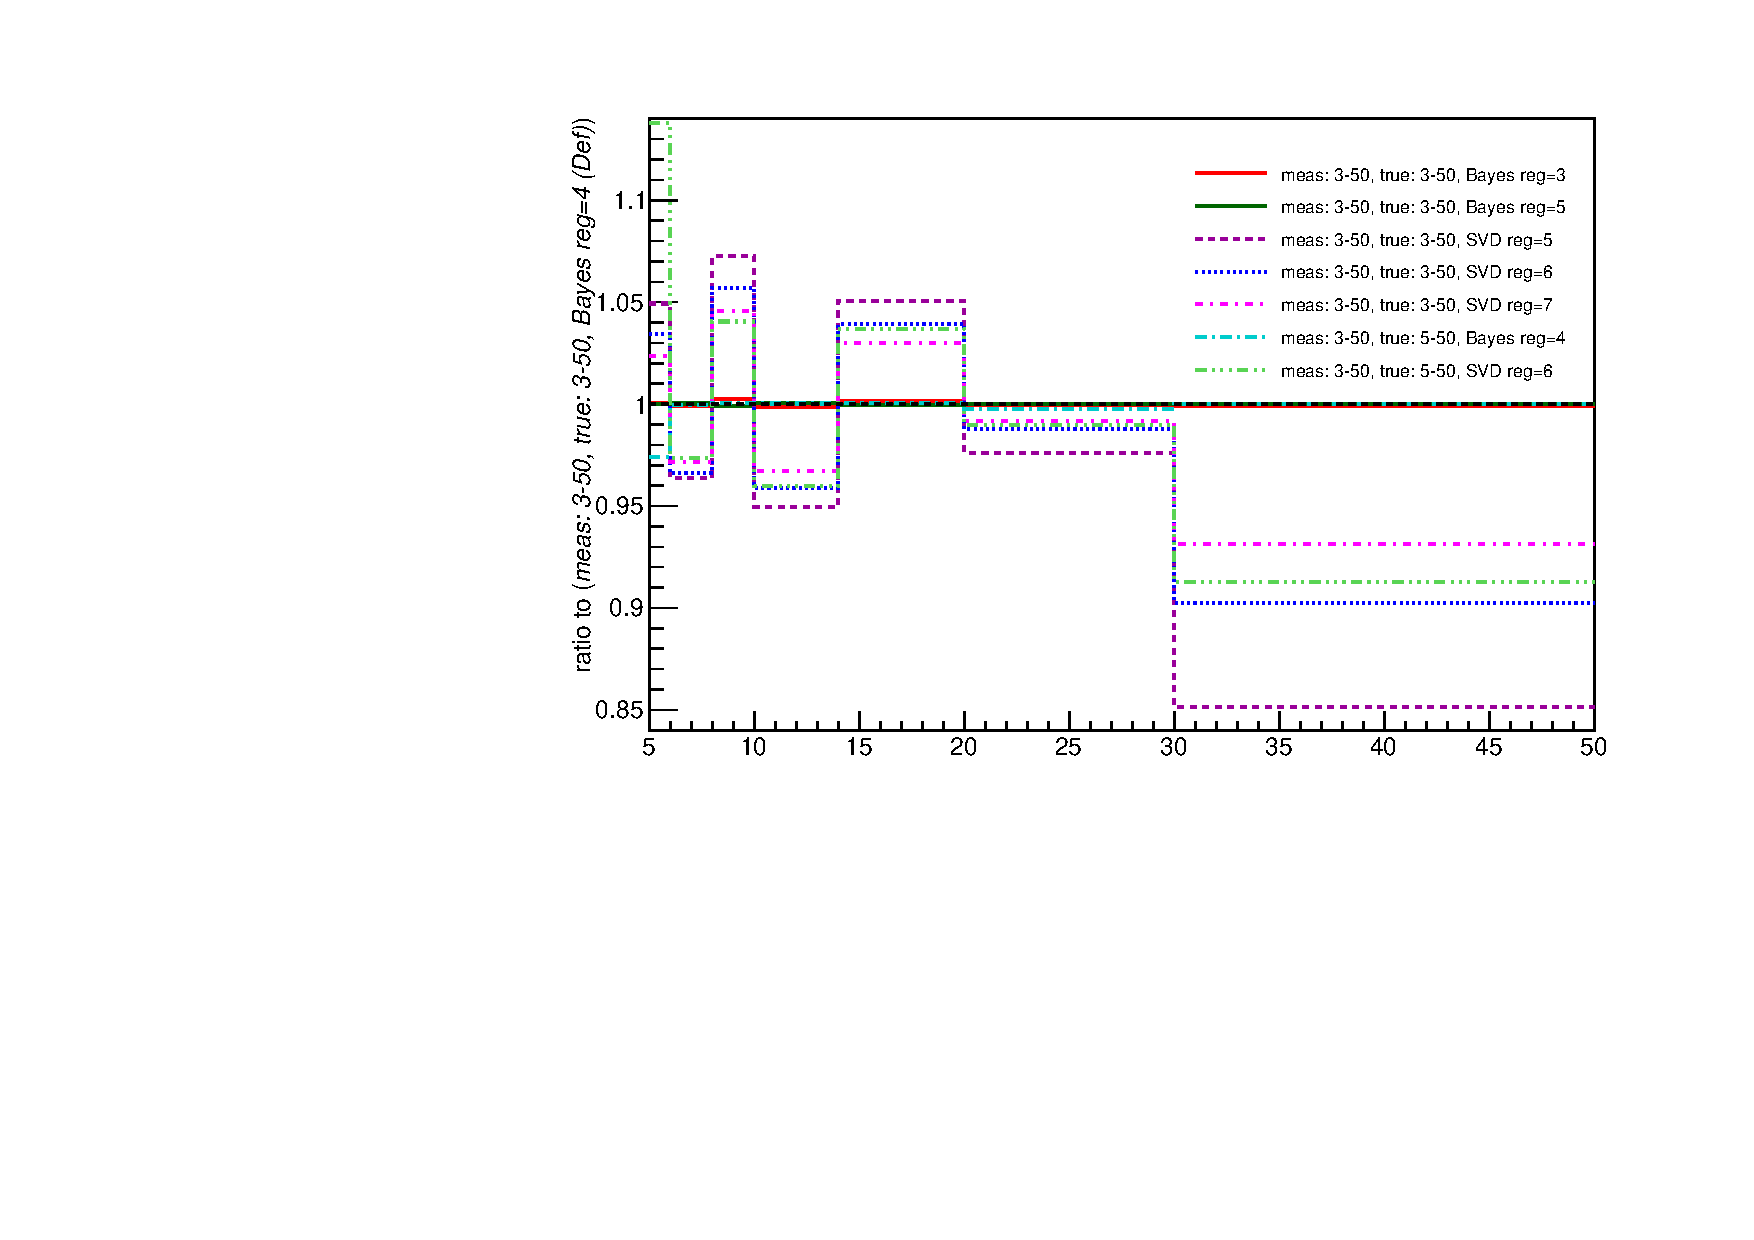
\includegraphics[width=0.49\textwidth]{pPbplotsD0/Default_jetMeas3_50_jetTrue3_50_PbPbbinning/systematics/UnfoldingRangesComparison_ratio.pdf}
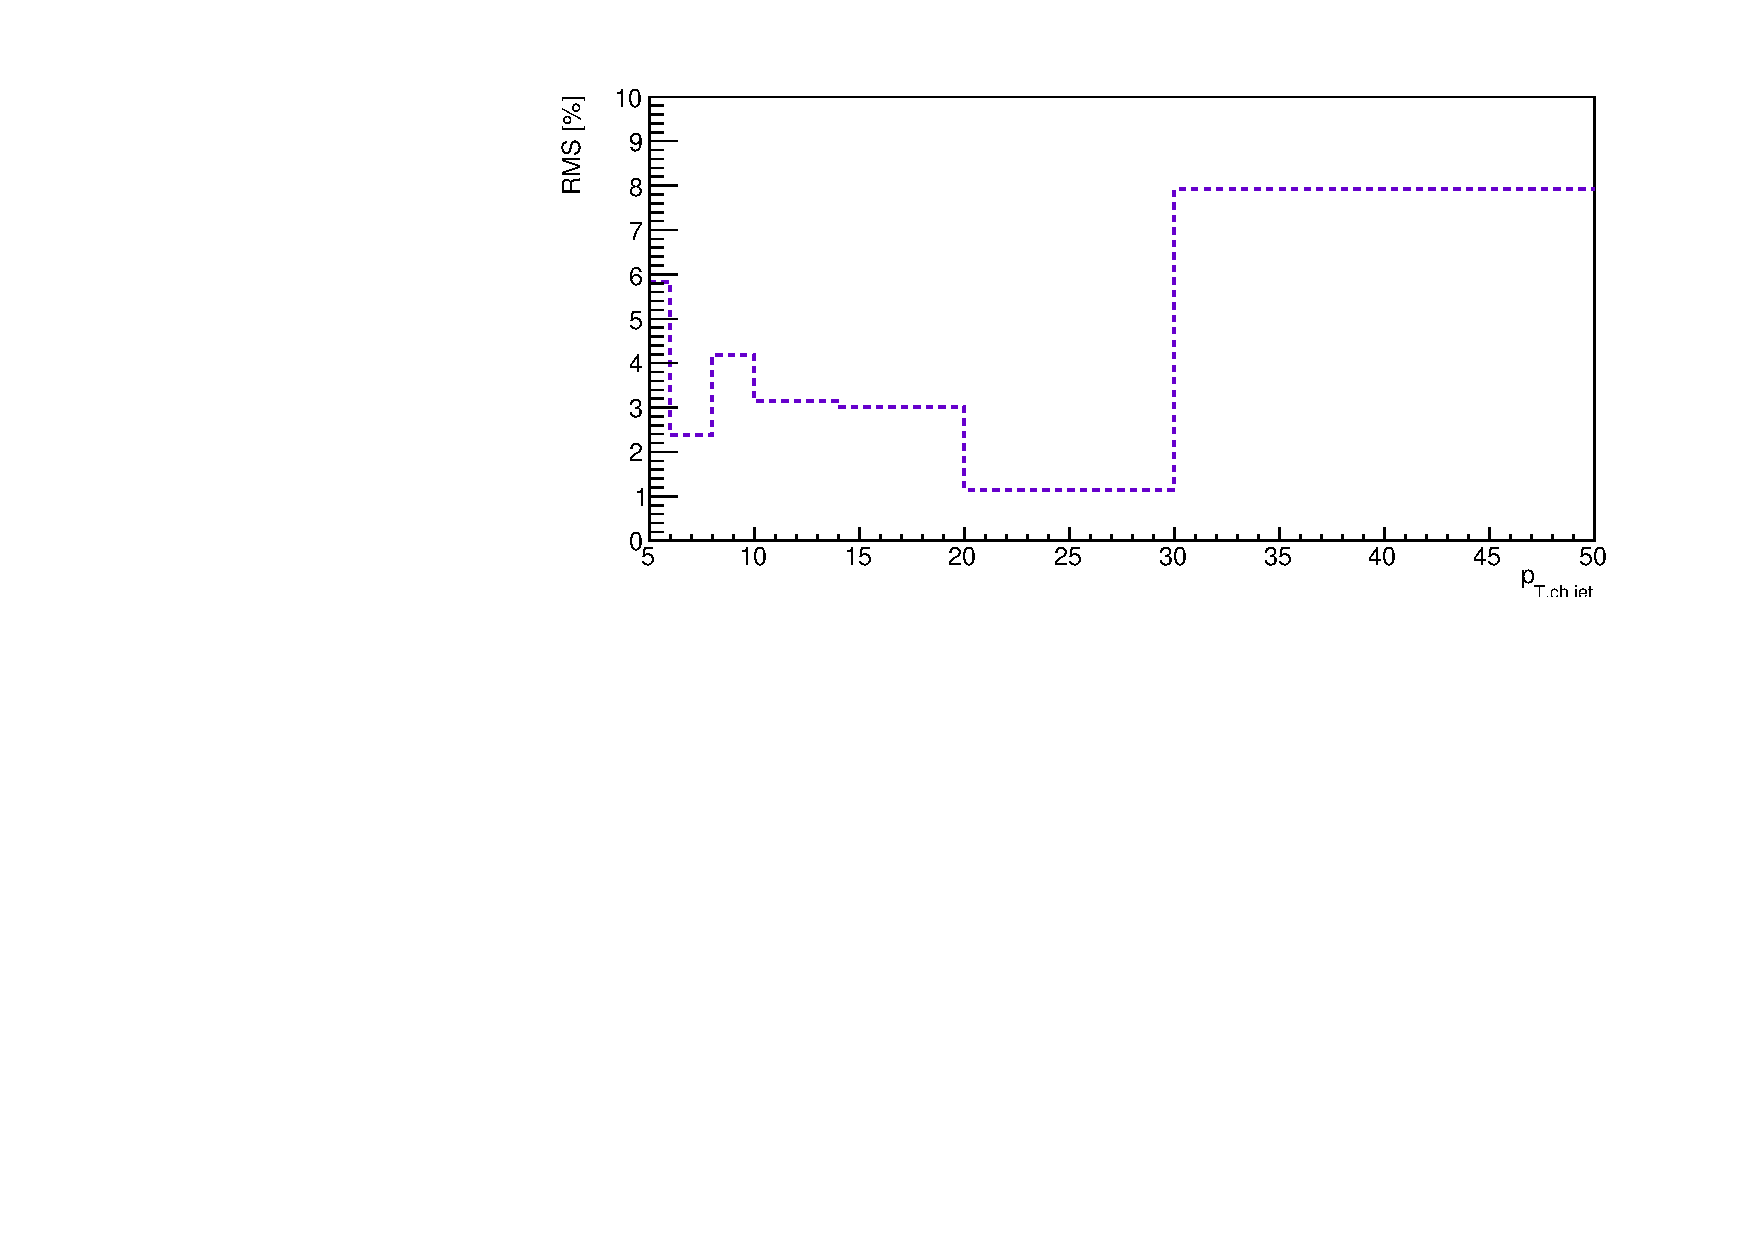
\includegraphics[width=0.49\textwidth]{pPbplotsD0/Default_jetMeas3_50_jetTrue3_50_PbPbbinning/systematics/UnfoldingRangesComparison_rms.pdf}
\caption{Ratio of unfolded \Dzero-jet \pt\ spectra with different ranges of $p_{T,jet}^{reco}$ and $p_{T,jet}^{gen}$ using Bayesian and SVD unfolding methods with different iterations (left) and systematic uncertanties from the RMS (right).}
\label{fig:PbPb_UnfSpec_pPb_Dzero_ranges}
\end{figure}

%\begin{itemize}
%\item 3 $<  p_{T,jet}^{reco} < $ 50, 3 $<  p_{T,jet}^{gen} < $ 50 -- \textbf{Default}
%\item 3 $<  p_{T,jet}^{reco} < $ 50, 5 $<  p_{T,jet}^{gen} < $ 50
%\item 4 $<  p_{T,jet}^{reco} < $ 50, 5 $<  p_{T,jet}^{gen} < $ 50
%\item 5 $<  p_{T,jet}^{reco} < $ 50, 5 $<  p_{T,jet}^{gen} < $ 50
%\end{itemize}

Figure~\ref{fig:PbPb_UnfSpec_pPb_Dzero_reg4} (left) shows unfolded jet \pt spectrum using Bayesian unfolding with 4 iterations (left) and unfolded spectra with next iterations compared to the default spectrum obtained after 4 iterations (right).
Unfolded spectrum with SVD method using 7 interation is presented in Fig.~\ref{fig:PbPb_UnfSpec_pPb_Dzero_SVD} (left) togehter with ratio of the refoleded spectra to the measured one (right).

\begin{figure}[bth]
\centering
\includegraphics[width=0.49\textwidth]{pPbplotsD0/Default_jetMeas3_50_jetTrue3_50_PbPbbinning/unfolding_Bayes_4/plots/unfoldedSpectrum_UnfSpectrum.pdf}
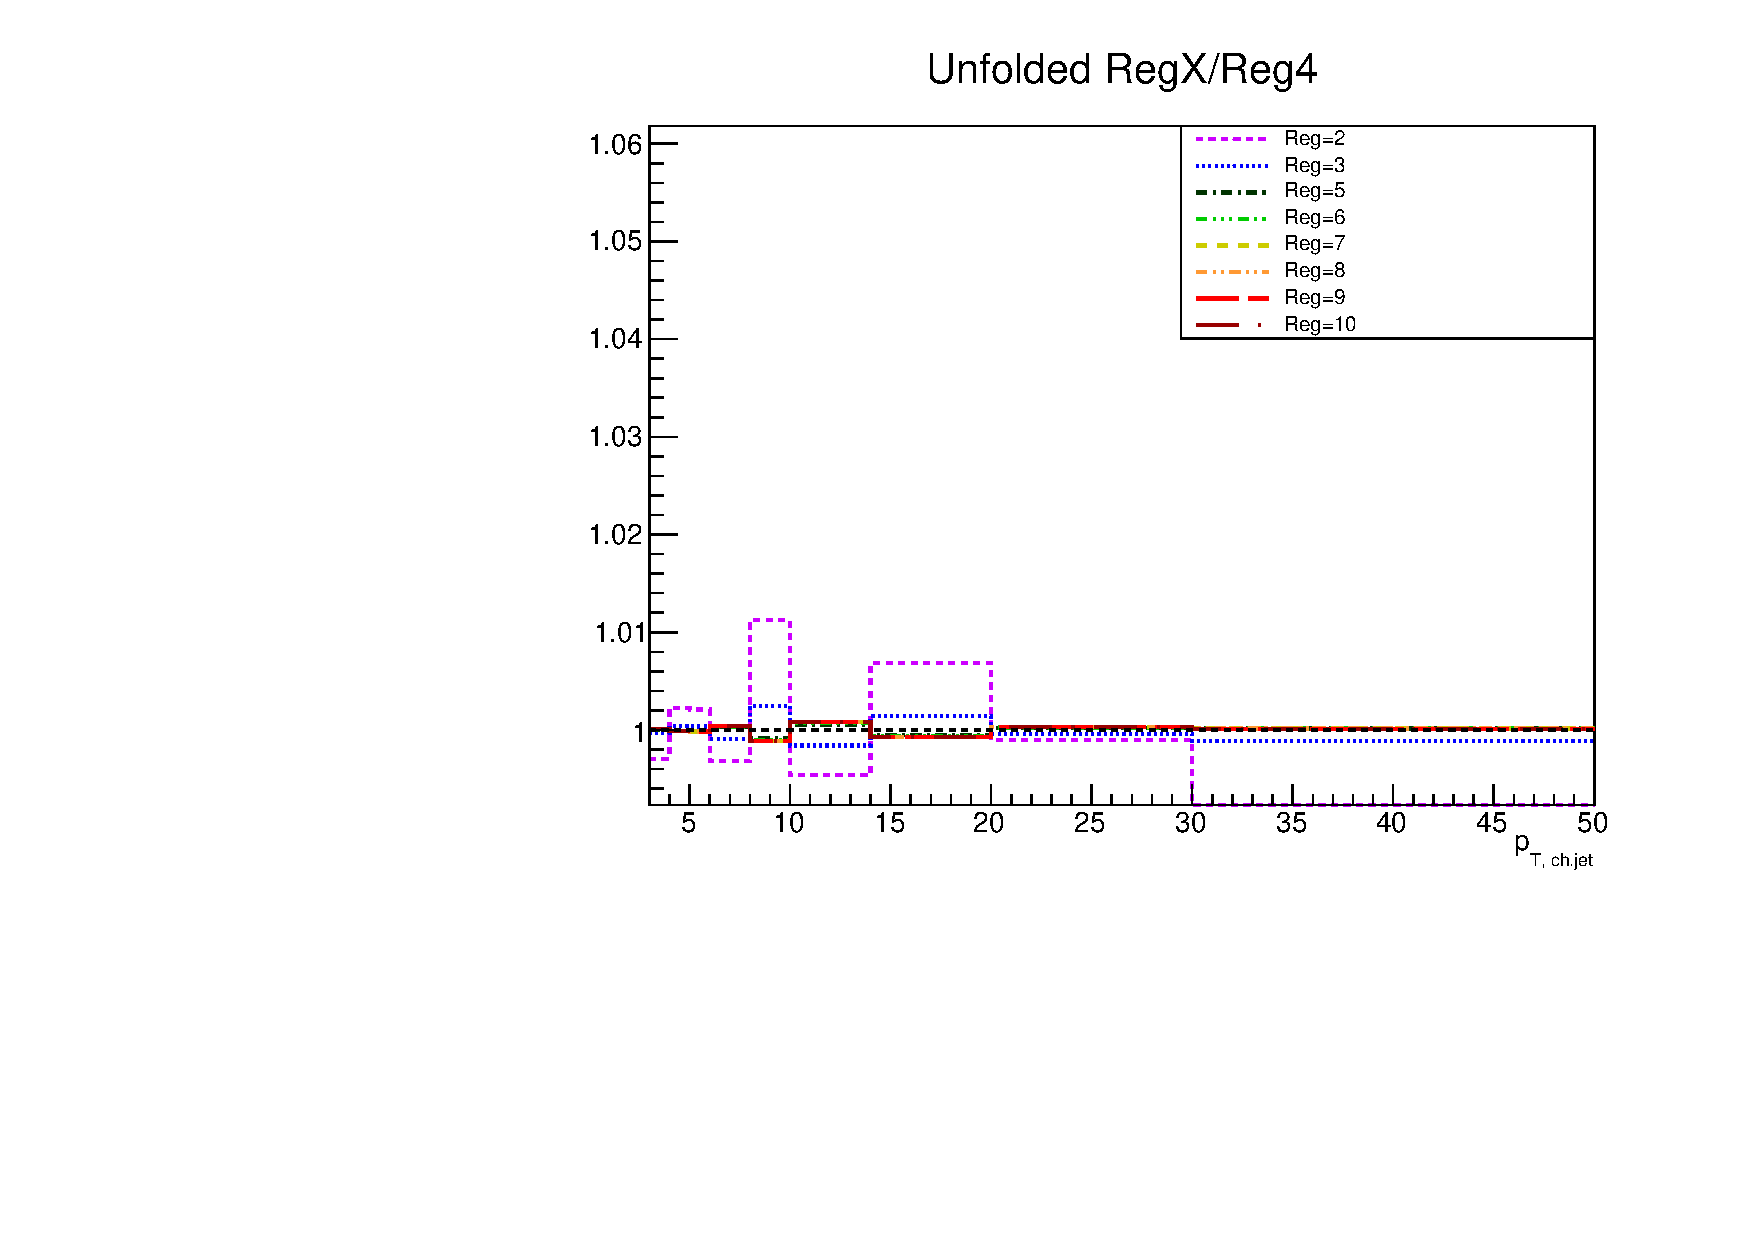
\includegraphics[width=0.49\textwidth]{pPbplotsD0/Default_jetMeas3_50_jetTrue3_50_PbPbbinning/unfolding_Bayes_4/plots/unfoldedSpectrum_unfRatio.pdf}
\caption{Left: Corrected jet \pt spectrum before (blue) and after (red) the unfolding procedure (Bayesian method with 4 iterations), \pPb\ events at $\snn=5.02$~TeV. Right: Ratio of the default unfolded spectrum with 4 iteration to the unfolded spectra for up to 10 iterations in the Bayesian unfolding. The considered jet \pt\ range is above 5 GeV/$c$.}
\label{fig:PbPb_UnfSpec_pPb_Dzero_reg4}
\end{figure}

\begin{figure}[bth]
\centering
\includegraphics[width=0.51\textwidth]{pPbplotsD0/Default_jetMeas3_50_jetTrue3_50_PbPbbinning/unfolding_SVD_7/plots/unfoldedSpectrum_UnfSpectrum.pdf}
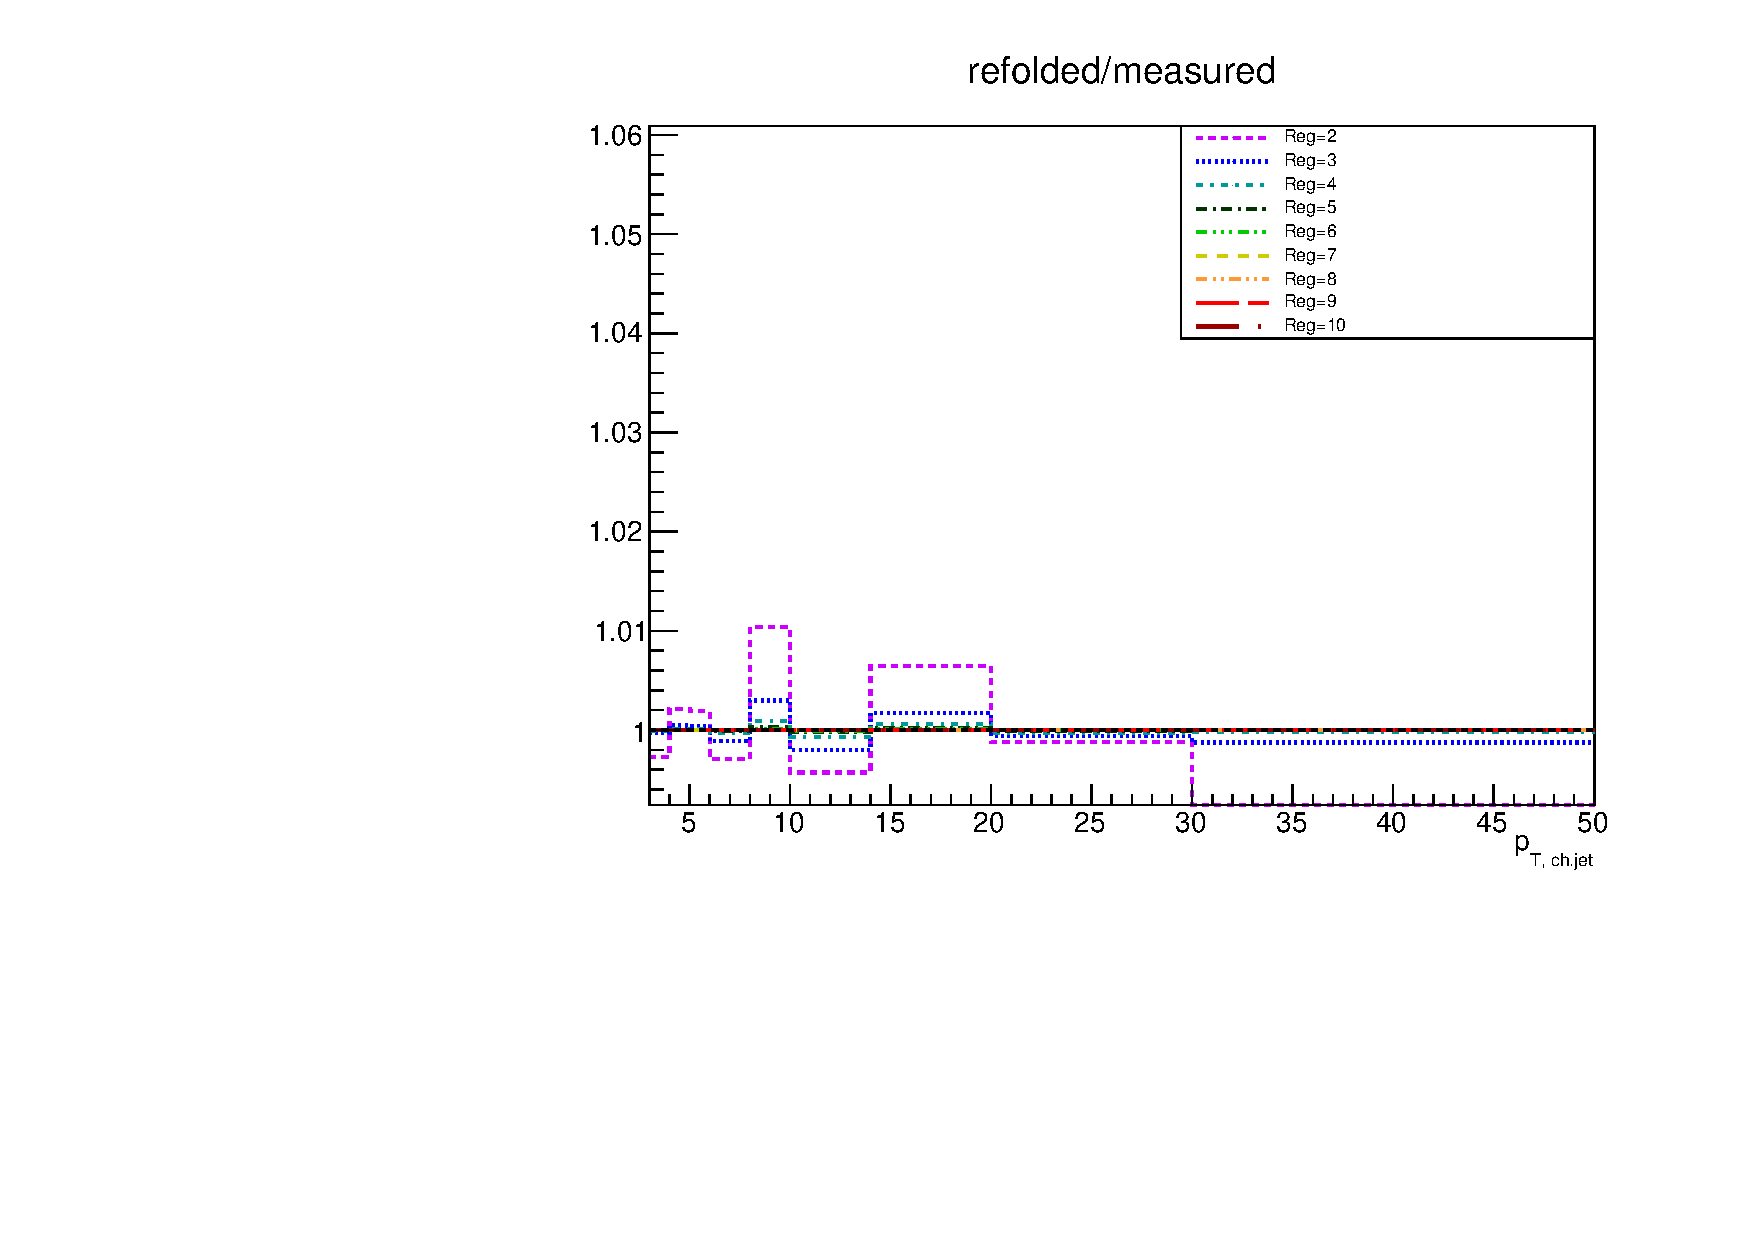
\includegraphics[width=0.48\textwidth]{pPbplotsD0/Default_jetMeas3_50_jetTrue3_50_PbPbbinning/unfolding_SVD_7/plots/unfoldedSpectrum_foldedRatio.pdf}
\caption{Left: Corrected jet \pt spectrum before (blue) and after (red) the unfolding procedure (SVD method with 7 iterations), \pPb\ events at $\snn=5.02$~TeV. Right: ratio of the measured spectrum to the refolded for up to 10 iterations in the SVD unfolding. The considered jet \pt\ range is above 5 GeV/$c$.}
\label{fig:PbPb_UnfSpec_pPb_Dzero_SVD}
\end{figure}


\begin{figure}[bth]
\centering
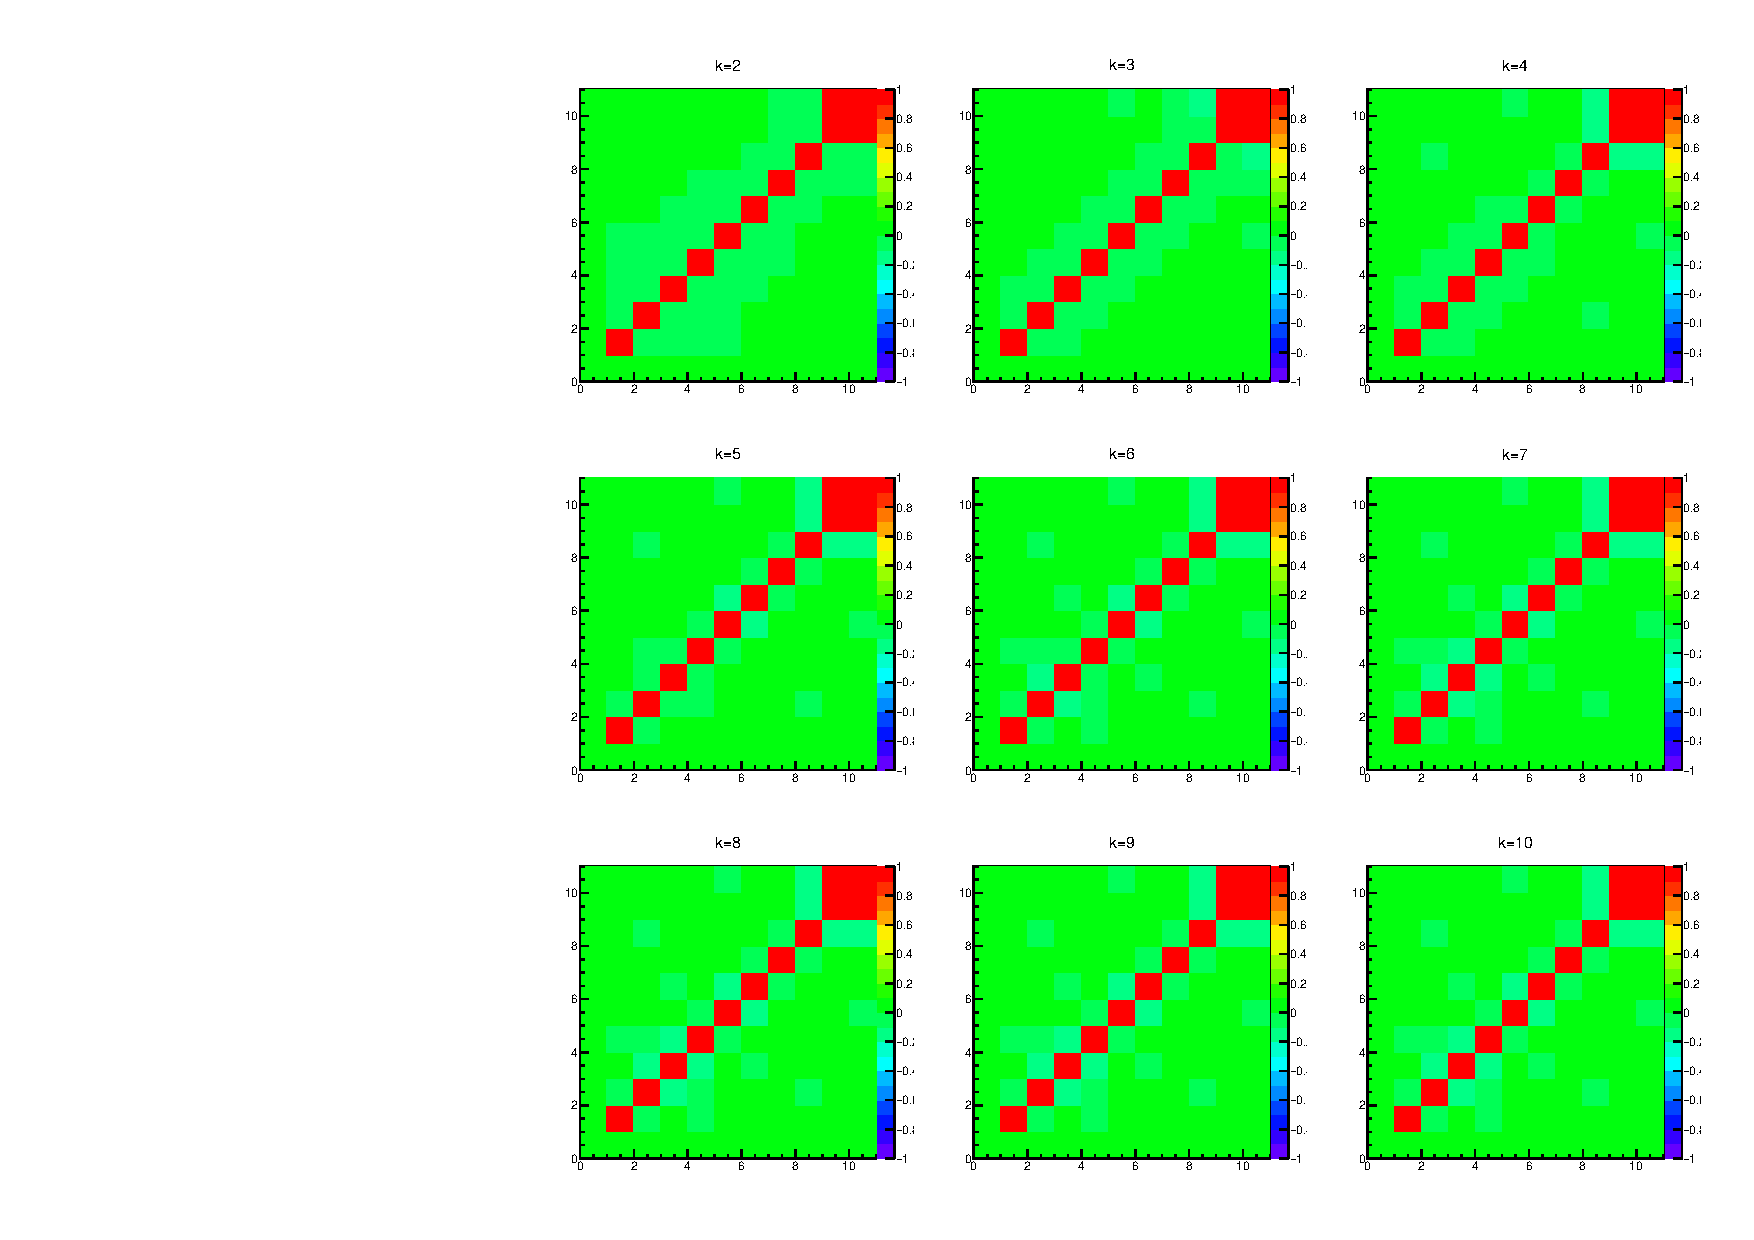
\includegraphics[width=0.8\textwidth]{pPbplotsD0/Default_jetMeas3_50_jetTrue3_50_PbPbbinning/unfolding_SVD_6/plots/unfoldedSpectrum_Pearson.pdf}
\caption{Pearson coefficients for SVD unfolding.}
\label{fig:PbPb_unfPearson_pPb_Dzero_SVD}
\end{figure}


The baseline prior used for unfolding is the spectrum obtained (at the generator level) from PYTHIA.
For the variations, the priors were obtained from a modified power-law function:
\begin{equation}
f(\ptjet) = \ptjet^{-a}e^{-\frac{ab}{\ptjet}},
\end{equation}
where $a$ is the power-law index and $b$ is the position of the local maximum of the distribution. The exponential factor $e^{-\frac{ab}{\ptjet}}$ was added to avoid infinities at zero and have a more realistic spectrum (the physical cross-section goes to zero for $\ptjet \to 0$).
Used variations are: %(we used two variations: $a=3,6$) 
\begin{itemize}
\item prior0: $a=4.6$ $b=4$~\GeVc\ 
\item prior1: $a=3$ $b=4$~\GeVc\
\item prior2: $a=4$ $b=4$~\GeVc\
\item prior3: $a=5$ $b=4$~\GeVc\
\item prior4: $a=6$ $b=4$~\GeVc\
\item prior5: $a=7$ $b=4$~\GeVc\
\item prior6: $a=4.5$ $b=3$~\GeVc\
\item prior7: $a=4.5$ $b=5$~\GeVc\
\item prior8: fit to the measured spectrum
\end{itemize}

Example of priors compared to the PYTHIA \Dzero-jet \pt\ spectra at the generator level are shown on Fig
Ratios of the unfolded \Dzero-jet \pt\ spectra with variation of the functions used as priors to the central \Dzero-jet \pt\ spectrum using the Bayesian unfolding with 3 (left) and 4 (right) iterations are shown in Fig.~\ref{fig:PbPb_UnfSpec_pPb_Dzero_priors}. 


\begin{figure}[bth]
\centering
\includegraphics[width=0.49\textwidth]{pPbplotsD0/Default_jetMeas3_50_jetTrue3_50_PbPbbinning/systematics/PriorComparison_reg3_ratio.pdf}
\includegraphics[width=0.49\textwidth]{pPbplotsD0/Default_jetMeas3_50_jetTrue3_50_PbPbbinning/systematics/PriorComparison_reg4_ratio.pdf}
\caption{Unfolded \Dzero-jet \pt\ spectra with different priors used in the unfolding procedure, using Bayes unfolding method with 3 (left) and 4 (right) iterations.}
\label{fig:PbPb_UnfSpec_pPb_Dzero_priors}
\end{figure}


\subsection{Background fluctuation matrix}
\label{sec:sysUnc_bkgFluctuations}


\subsubsection{\Dzero-tagged jets}
The same procedure is followed in the \Dzero-jet analysis, with R=0.3.
In addition to the cases used before, following new requirement are considered:
\begin{itemize}
\item Events with \Dzero-jet candidates and with $p_{T, lead}>$ 5 GeV/$c$, excluding the leading jet from the Random Cone, the leading jet is defined as a jet with the highest \pt\ in an event. \textbf{Default}
\item Events with \Dzero-jet candidates and with $p_{T, lead}>$ 5 GeV/$c$, excluding the leading jet from the Random Cone, the leading jet is defined as a \Dzero-jet candidate.
\item Events with \Dzero-jet candidates and with $p_{T, lead}>$ 5 GeV/$c$, Random Cone is placed in the perpendicular plane to the leading jet, the leading jet is defined as a jet with the highest \pt\ in an event.
\item Events with \Dzero-jet candidates and with $p_{T, lead}>$ 5 GeV/$c$, Random Cone is placed in the perpendicular plane to the leading jet, the leading jet is defined as a \Dzero-jet candidate.
\item Events with \Dzero-jet candidates and with $p_{T, lead}>$ 10 GeV/$c$, excluding the leading jet from the Random Cone, the leading jet is defined as a jet with the highest \pt\ in an event.
\item Events with \Dzero-jet candidates and with $p_{T, lead}>$ 10 GeV/$c$, excluding the leading jet from the Random Cone, the leading jet is defined as a \Dzero-jet candidate.
\item Events with \Dzero-jet candidates and with $p_{T, lead}>$ 10 GeV/$c$, Random Cone is placed in the perpendicular plane to the leading jet, the leading jet is defined as a jet with the highest \pt\ in an event.
\item Events with \Dzero-jet candidates and with $p_{T, lead}>$ 10 GeV/$c$, Random Cone is placed in the perpendicular plane to the leading jet, the leading jet is defined as a \Dzero-jet candidate.
\item All events with $p_{T, lead}>$ 5 GeV/$c$, excluding the leading jet from the Random Cone, the leading jet is defined as a jet with the highest \pt\ in an event. 
\item All events with $p_{T, lead}>$ 5 GeV/$c$, Random Cone is placed in the perpendicular plane to the leading jet, the leading jet is defined as a jet with the highest \pt\ in an event.
\item All events with $p_{T, lead}>$ 10 GeV/$c$, excluding the leading jet from the Random Cone, the leading jet is defined as a jet with the highest \pt\ in an event. 
\item All events with $p_{T, lead}>$ 10 GeV/$c$, Random Cone is placed in the perpendicular plane to the leading jet, the leading jet is defined as a jet with the highest \pt\ in an event.
\end{itemize}
It gives it total 12 background fluctuations matrices, where the matrix from~\ref{sec:BackFluc} is used as the default in the analysis and the rest of them are used to estimate the systematic uncertainty. 




Base on these \deltapt\ distributions, new background fluctuation matrices are build. They are then used to build a combined prompt response matrix and the measured \Dzero-jet\ \pt spectrum is unfolded. Ratios of the unfolded spectra and RMS are shown in Fig.~\ref{fig:PbPb_BkgFlucSys_Dzero}.

\begin{figure}[bth]
\centering
\includegraphics[width=0.49\textwidth]{pPbplotsD0/Default_jetMeas3_50_jetTrue3_50_PbPbbinning/systematics/BkgComparison_reg3_ratio.pdf}
\includegraphics[width=0.49\textwidth]{pPbplotsD0/Default_jetMeas3_50_jetTrue3_50_PbPbbinning/systematics/BkgComparison_reg3_rms.pdf}
\caption{ Left Ratio of unfolded \Dzero-jet \pt\ spectra with different background fluctuation matrices. Right: systematic unceranties from RMS.}
\label{fig:PbPb_BkgFlucSys_Dzero}
\end{figure}


\subsection{Tracking Efficiency}
%For this dataset the uncertainty on the tracking efficiency is estimated to be about 5\%, based on past studies.
Uncertainties on the tracking efficiency affect the measurement in two ways. 

First, it introduces an uncertainty on the D-meson reconstruction efficiency. This was evaluated for the D-meson spectra to be 4-4.5\% for \Dstar\ and 3\% for \Dzero\ (mostly \pt-independent). Since we have verified that the reconstruction efficiency itself does not depend on \ptchjet\ we can assume that our measurement is affected by the same uncertainty.

\subsection{Tracking Efficiency -- Jet Energy Scale}

\subsubsection{\Dzero-tagged jets}

Tracking efficiency also affects the detector response. To estimate the uncertainty on the final yield, a new detector response has been built where the efficiency has been reduced to 96\% of its normal value, by throwing randomly away 4\% of the reconstructed track in the simulation.
The raw spectrum is unfolded using this modified response matrix and the outcome is compared with the reference result. The resulting systematic uncertainty is presented in Fig.~\ref{fig:PbPb_JESsys_Dzero}. As a cross-check of the observed effect the efficiency was also reduced to 95\%, the value used for the previous pp analysis - the found uncertainties agree between the two analysis. 
The three cases, of 4, 5 and 10\% inefficiency are fitted in order to check linearity, the quoted uncertainty is assumed to be symmetric. 
The systematic uncertainty is estimated by fitting the ratio and as the uncertainty the value obtained from the fitted function is used, the final systematic uncertanties are shown in Fig.~\ref{fig:PbPb_JESsys_Dzero}.

\begin{figure}[bth]
\centering
\includegraphics[width=0.49\textwidth]{pPbplotsD0/Default_jetMeas3_50_jetTrue3_50_PbPbbinning/systematics/JES_reg3.pdf}
\includegraphics[width=0.49\textwidth]{pPbplotsD0/Default_jetMeas3_50_jetTrue3_50_PbPbbinning/systematics/JES_reg3_ratio.pdf}
\caption{Unfolded \Dzero-jet spectra (left) and a ratio (right) between default unfolding result and with reduced tracking efficiency to 96 and 95\%.}
\label{fig:PbPb_JESsys_Dzero}
\end{figure}


\begin{figure}[bth]
\centering
\includegraphics[width=0.55\textwidth]{pPbplotsD0/Default_jetMeas3_50_jetTrue3_50_PbPbbinning/systematics/JES_reg3_unc.pdf}
\caption{Systematic uncertainty from the JES, for 4, 5 and 10\% inefficiency on \Dzero-jet spectra. The final uncertainty is taken from the 96\% efficiency case. }
\label{fig:PbPb_JESsys_Dzero}
\end{figure}


\subsection{Summary of Systematic Uncertainties}


\subsubsection{\Dzero-tagged jets}

The summary of all uncertainties, including statistical uncertainties are listed for all \ptchjet\ bins of the final spectrum in Table~\ref{tab:UncSum_Dzero_PbPb}.
Figure~\ref{fig:PbPb_SysUnce_Dzero} shows all relative systematic uncertainties as a function of \ptchjet.

\begin{figure}[bth]
\centering
\includegraphics[width=.65\textwidth]{/home/basia/Work/alice/analysis/alice_Djets/analysisNote_pPbQM18/pPbplotsD0/Default_jetMeas3_50_jetTrue3_50_PbPbbinning/unfolding_Bayes_3/finalSpectra/plots/JetPtSpectra_allUnc.pdf}
\caption{\Dzero-jet\ systematic uncertanties in \pPb\ collisions at $\snn=5.02$~TeV.}
\label{fig:PbPb_SysUnce_Dzero}
\end{figure}

    \begin{table}[bth]
\caption{\Dzero-jet: Summary of all uncertainties.}
     \label{tab:UncSum_Dzero_PbPb}
\begin{center}
    \begin{tabular}{lrrrrrr}
    \hline
Source & \multicolumn{6}{c}{Uncertainty (\%)} \\ \hline
\ptchjet\ (\GeVc) & 5 - 10 & 10 - 15 & 15 - 20 & 20 - 25 & 25 - 35 & 35 - 50 \\ \hline
Raw Yield Extraction & 2 & 2 & 3 & 5 & 5 & 7  \\
Reflections & 1 & 1 & 1 & 4 & 1 & 1  \\
Side-Band and Signal ranges & 2 & 1  & 4 & 2 & 8 & 10  \\
Selection Cuts & 4 & 4 & 4 & 10 & 10 & 10  \\
B Feed-Down & 7 & 7 & 9 & 14 & 15 & 12  \\
Unfolding: priors & 4 & 5 & 5 & 2 & 3 & 9  \\
Unfolding: ranges, SVD & 6 & 2 & 2 & 1 & 3 & 3  \\
Bkg. fluct. matrix & 2 & 3 & 2 & 1 & 1 & 1  \\
Tracking Eff. (D-Meson) & 3 & 3 & 3 & 3 & 3 & 3 \\
Tracking Eff. (Jet Energy Scale) & 1  & 2 & 4 & 6 & 8 & 12  \\
\hline
Total Systematic Uncertainty & 12 & 12 & 14 & 20 & 23 & 26  \\
\hline
Normalization Uncertainty & \multicolumn{6}{c}{ 3.8 } \\
\hline
Statistical & 2 & 5 & 9 & 18 & 20 & 29  \\
\hline
    \end{tabular}
    \end{center}
    \end{table}
    


%%%%%%%%%%%%%%%%%%%%%%%%%%%%%%%%%%%%%%%%%%%%%%%%%%%%%%%%%%%%%%%%%%%%%%
%%%%%%%%%%%%%%%%%%%%%%%%%%%%%%%%%%%%%%%%%%%%%%%%%%%%%%%%%%%%%%%%%%%%%%
%%%%%%%%%%%%%%%%%%%%%%%%%%%%              RESULTS              %%%%%%%%%%%%%%%%%%%%%%%%%%%%
%%%%%%%%%%%%%%%%%%%%%%%%%%%%%%%%%%%%%%%%%%%%%%%%%%%%%%%%%%%%%%%%%%%%%%
%%%%%%%%%%%%%%%%%%%%%%%%%%%%%%%%%%%%%%%%%%%%%%%%%%%%%%%%%%%%%%%%%%%%%%

\section{Results}


This Section contains a summary of the results.
The  $D$-jet \pt-differential cross-section in \pPb\ collisions at $\snn=5.02$~TeV  with all corrections applied (reconstruction efficiency, B feed-down subtraction, unfolding for detector momentum resolution);
The cross-section is calculated according to the following formula:
\begin{equation}
\frac{{\rm d}^2\sigma}{{\rm d}\eta {\rm d}\pt}=\frac{1}{L_{\rm int}f_{\rm BR}} \frac{N_{\rm D-jets}(\ptjet)}{\Delta\ptjet\Delta\eta},
\end{equation}
where $L_{\rm int}=N_{\rm evt}/\sigma_{\rm inel}$ is the integrated luminosity ($\sigma_{\rm pPb, inel} = 2.09$~b), $f_{\rm BR}$ is the branching
ratio of the D-meson decay channel used in the analysis, $N_{\rm D-jets}(\ptjet)$ is the measured number of D-jets in a given \ptjet\ bin (with all corrections applied).


The $D^{0}$-tagged jet \pt\ differential cross section in \pPb\ collisions at $\snn=5.02$~TeV compared to PYTHIA+POWHEG prediction is shown in Fig~\ref{fig:PbPb_pPbJetPt_final_D0}.
\begin{figure}[bth]
\centering
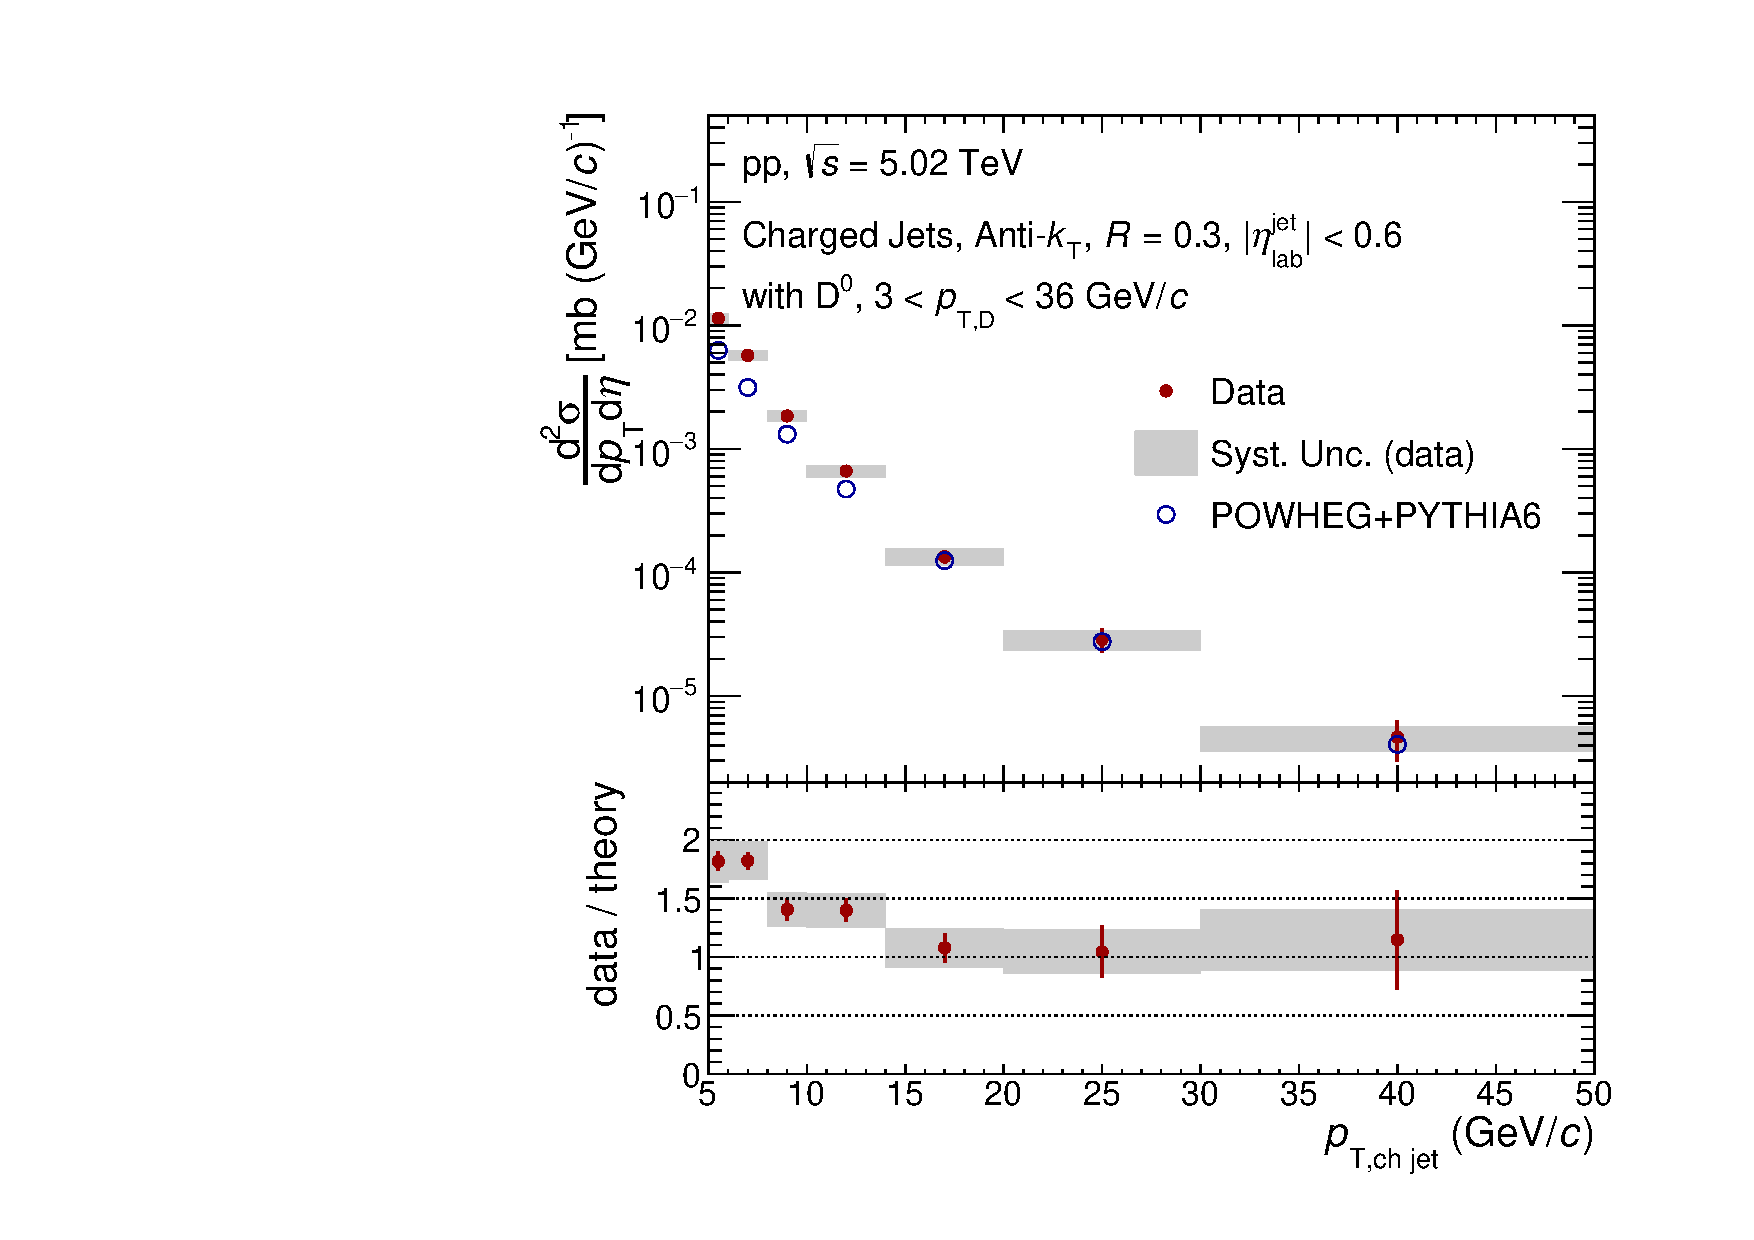
\includegraphics[width=.8\textwidth]{/home/basia/Work/alice/analysis/alice_Djets/analysisNote_pPbQM18/pPbplotsD0/Default_jetMeas3_50_jetTrue3_50_PbPbbinning/unfolding_Bayes_3/finalSpectra/plots/JetPtSpectra_final.pdf}
\caption{Unfolded \Dzero-jet\ spectrum in \pPb\ collisions at $\snn=5.02$~TeV compared to PYTHIA+POWHEG simulations, with the simulation uncertainty.}
\label{fig:PbPb_pPbJetPt_final_D0}
\end{figure}


